\section{Fundamentos de Ecuaciones Diferenciales}

\subsection{Conceptos básicos}

\begin{definicion}
	\begin{itemize}
	\item 	Una \emph{ecuación diferencial} es una ecuación que involucra derivadas o diferenciales de una o varias variables.
	\item Si la ecuación sólo involucra derivadas respecto a una única variable independiente, diremos que es \emph{ordinaria}.  En otro caso, que es \emph{parcial}.
	\item Si la ecuación involucra derivadas de orden $n$, pero no de orden más alto, diremos que la propia ecuación es de \emph{orden $n$.}
\end{itemize}
\end{definicion}

\begin{resuelto}
	Clasifica cada una de las siguientes ecuaciones diferenciales enunciando su orden; sus variables dependientes e independientes; y si es ordinaria o parcial:

\begin{align}
	x^2y''+xy'+\left(x^2-n^2\right)y = 0
\end{align}

\begin{proof}[Solución]
	\begin{enumerate}[(i)]
		\item Orden 2;
		\item variable dependiente: $ y $;
		\item variable independiente: $ x $;
		\item ecuación ordinaria.
	\end{enumerate}
\end{proof}



\begin{align}
	\dfrac{dx}{dy}= x^{2}+y^{2}
\end{align}
\begin{proof}[Solución]
	\begin{enumerate}[(i)]
		\item Orden 1;
		\item variable dependiente: $ x $;
		\item variable independiente: $ y $;
		\item ordinaria.
	\end{enumerate}
\end{proof}



\begin{align}
	\dfrac{dy}{dx}= \dfrac{1}{x^{2}+y^{2}}
\end{align}
\begin{proof}[Solución]
	\begin{enumerate}[(i)]
		\item Orden 1;
		\item variable dependiente: $ y $;
		\item variable independiente: $ x $;
		\item ordinaria.
	\end{enumerate}
\end{proof}



\begin{align}
	\left(\dfrac{d^{2}u}{dt^{2}}\right)^{3}+u^{4}=1
\end{align}
\begin{proof}[Solución]
	\begin{enumerate}[(i)]
		\item Orden 2;
		\item variable dependiente: $ u $;
		\item variable independiente: $ t $;
		\item ordinaria.
	\end{enumerate}
\end{proof}




\begin{align}
	\dfrac{\partial^{2}Y}{\partial t^{2}} = 2\dfrac{\partial^{2}Y}{\partial x^{2}}
\end{align}
\begin{proof}[Solución]
	\begin{enumerate}[(i)]
		\item Orden 2;
		\item variable dependiente: $ Y $;
		\item variables independientes: $ x,t $;
		\item parcial.
	\end{enumerate}
\end{proof}




\begin{align}
	\left(x^{2}+2y^{2}\right)dx +\left(3x^{3}-4y^{2}\right)dy=0
\end{align}
\begin{proof}[Solución]
	\begin{enumerate}[(i)]
		\item Orden 1;
		\item variable dependiente: $ y  $;
		\item variable independiente: $ x $;
		\item ordinaria.
	\end{enumerate}
\end{proof}


\end{resuelto}


	\begin{definicion}
		Una constante arbitraria es un valor que es independiente de las variables involucradas en la ecuación.
	\end{definicion}

	\begin{observacion}
		Generalmente las denotaremos con las primeras letras del alfabeto:
	\begin{align}
		A,B,C,c_{1},c_{2},...
	\end{align}
	\end{observacion}

%%%%

	\begin{ejemplo}
		En la ecuación
		\begin{align}
		y = x^{2}+c_{1}x+c_{2}
		\end{align}
		los símbolos $ c_{1}, c_{2} $ representan constantes arbitrarias.

	\end{ejemplo}



	\begin{ejemplo}
		La relación $ y = Ae^{-4x+B} $ se puede reescribir como $ y = Ce^{-4x} $.  Por lo que sólo involucra una constante arbitraria.
	\end{ejemplo}


\begin{observacion}

	Siempre reduciremos las ecuaciones al número mínimo de constantes arbitrarias, a las que llamaremos \emph{esenciales}.

\end{observacion}
%%%


\subsection{Soluciones de ecuaciones diferenciales}

\begin{itemize}
	\item 	Una \emph{solución de una ecuación diferencial} es una relación entre las variables que está libre de derivadas, y que satisface la ecuación diferencial en al menos un intervalo.
	\item
	Una \emph{solución general} de una ecuación diferencial de orden $ n $ es aquella que involucra $ n $ constantes arbitrarias esenciales.
	\item 	Una \emph{solución particular} es aquella que se obtiene de una general, sustituyendo valores específicos en las constantes arbitrarias.
	\item 	Una \emph{solución singular} es una aquella que no se puede obtener de la solución general sólo especificando valores para las constantes arbitrarias.
\end{itemize}



	\begin{resuelto}
		\label{exmp 02:06}
		Demuestra que $ y=x^{2}+c_{1}x+c_{2} $ es una solución general de $ y''=2 $.
	\end{resuelto}

	\begin{resuelto}
		\label{exmp 02:08}
		Verifica que $ y = x^2-3x+2 $ es una solución particular de $ y''=2 $.
	\end{resuelto}

	\begin{ejemplo}
		La solución general de $ y = xy'-y'^{2} $ es $ y = cx-c^{2} $.

		 Sin embargo, $ y=\dfrac{x^{2}}{4} $ es una solución que no se puede obtener sustituyendo $ c $.  Por tanto, es una solución particular.
	\end{ejemplo}


\begin{definicion}
	Una solución general de orden $ n $ tiene $ n $ parámetros (constantes arbitrarias esenciales) y por tanto, geométricamente representa una \emph{familia de curvas $n-$paramétrica. }

	De manera reciproca, una relación con $ n $ constantes arbitrarias (también llamada \emph{primitiva}) tiene asociada una ecuación diferencial de orden $n$ (de la cual es solución general), llamada la \emph{ecuación diferencial de la familia}.

\end{definicion}

\subsection{Ejemplos de soluciones}


Para cada una de las siguientes ecuaciones, verifica si la relación indicada es solución; y en ese caso, determina si es general.




\begin{align}
	\begin{cases}
		y'-x+y=0\\
		y = Ce^{-x}+x-1
	\end{cases}
\end{align}



\begin{proof}[Solución]
	\begin{enumerate}[(i)]
		\item $y'=-Ce^{-x}+1$
		\item $y'-x+y= (-Ce^{-x}+1)-x+(Ce^{-x}+x-1)=0$
		\item $C$ es su único parámetro.
		\item Por tanto $y$ es solución general.
	\end{enumerate}
\end{proof}



\begin{align}
	\begin{cases}
		\dfrac{dy}{dx}=\dfrac{2xy}{3y^{2}-x^{2}}\\
		x^{2}y-y^{3}=c
	\end{cases}
\end{align}



\begin{proof}[Solución]
	\begin{enumerate}[(i)]
		\item Derivando de forma implícita obtenemos
		\begin{align}
			x^{2}y'+2xy-3y^{2}y'=0
		\end{align}
		\item Despejando $y'$ obtenemos
		\begin{align}
			y'=\dfrac{2xy}{3y^{2}-x^{2}}
		\end{align}
		\item Como $C$ es el único parámetro, $y$ es una solución general.
	\end{enumerate}
\end{proof}



\begin{align}
	\label{problem 2.2:c}
	\begin{cases}
		\dfrac{d^{2}I}{dt^{2}}+2\dfrac{dI}{dt}-3I =
		2\cos(t)-4\sin(t)\\
		I = c_{1}e^{t}+c_{2}e^{-3t}+\sin(t)
	\end{cases}
\end{align}



\begin{proof}[Solución]
	\begin{enumerate}[(i)]
		\item $ \dfrac{dI}{dt}
		=c_{1}e^{t}-3c_{2}e^{-3t}+\cos(t) $

		\item $ \dfrac{d^{2}I}{dt^{2}} =
		c_{1}e^{t}+9c_{2}e^{-3t}-\sin(t) $

		\item
		\begin{align}
			\left(c_{1}e^{t}+9c_{2}e^{-3t}-\sin(t)\right)\\
			+2\left(c_{1}e^{t}-3c_{2}e^{-3t}+\cos(t)\right)\\
			-3\left(c_{1}e^{t}+c_{2}e^{-3t}+\sin(t)\right)\\
			=   2\cos(t)-4\sin(t)
		\end{align}

		\item Como $ c_{1},c_{2} $ son parámetros, entonces $I$ es una solución general.
	\end{enumerate}
\end{proof}



\begin{align}
	\begin{cases}
		x^{3}\left(\dfrac{d^{2}v}{dx^{2}}\right)^{2} = 2v\dfrac{dv}{dx} \\
		v = cx^{2}
	\end{cases}
\end{align}



\begin{proof}[Solución]
	\begin{enumerate}[(i)]
		\item $ \dfrac{dv}{dx}=2cx $
		\item $ \dfrac{d^{2}v}{dx^{2}}=2c $
		\item Sustituimos en el lado izquierdo
		\begin{align}
			x^{3}\left(2c\right)^{2}=4c^{2}x^{3}
		\end{align}
		\item Sustituimos en el lado derecho
		\begin{align}
			2\left(cx^{2}\right)\left(2cx\right)= 4c^{2}x^{3}
		\end{align}
		\item Entonces $v$ es solución, pero como la ecuación es de grado 2 y $c$ es el único parámetro, no es general.
	\end{enumerate}
\end{proof}



% PROBLEMA RESUELTO 2.3
\begin{resuelto}
	Determine la solución particular de la ecuación diferencia del problema \ref{problem 2.2:c}, tal que satisface las condiciones
	\begin{align}
		I(0)&=2\\
		I'(0)&=-5
	\end{align}
\end{resuelto}




\begin{proof}[Solución]
	\begin{enumerate}[(i)]
		%NUEVO ITEM
		\item $I(t)=c_{1}e^{t}+c_{2}e^{-3t}+\sin(t)$
		\item $I(0)= c_{1}+c_{2}=  2$
		\item $I'(t)= c_{1}e^{t}-3c_{2}e^{-3t}+\cos(t)$
		\item $I'(0)= c_{1}-3c_{2}+1= -5$
		\item $c_{1}-3c_{2}=-6$
		\item $c_{1}=0, c_{2}=1$
		\item $I= 2e^{-3t}+\sin(t)$
	\end{enumerate}
\end{proof}



% problema resuelto 2.4
\begin{resuelto}
	Mostrar que la solución de problema de valor inicial
	\begin{align}
		\begin{cases}
			Q''(t)+4Q'(t)+20Q(t)=16e^{-2t} & t\geq 0 \\
			Q(0) = 2, Q'(0)=0 &
		\end{cases}
	\end{align}
	is
	\begin{align}
		Q(t) = e^{-2t}\left(
		1+\sin(4t)+\cos(4t)
		\right)
	\end{align}
\end{resuelto}



{Solución}
\begin{align}
	Q'(t) &= e^{-2t}\left( 4\cos(4t)-4\sin(4t) \right)
	-2e^{-2t}\left( 1+\sin(4t)+\cos(4t) \right)\\
	&=e^{-2t}\left( 2\cos(4t)-6\sin(4t)-2 \right)
\end{align}


{Solución}
\begin{align}
	Q''(t) &= e^{-2t}\left( -8\sin(4t)-24\cos(4t) \right)
	-2e^{-2t}\left( 2\cos(4t)-6\sin(4t)-2 \right)\\
	& = e^{-2t}\left( 4\sin(4t)-28\cos(4t)+4 \right)
\end{align}



{Solución}
\begin{align}
	Q''(t)+4Q'(t)+20Q(t) \\
	=
	e^{-2t}\left( 4\sin(4t)-28\cos(4t)+4 \right) \\
	+4e^{-2t}\left( 2\cos(4t)-6\sin(4t)-2 \right) \\
	+20e^{-2t}\left(
	1+\sin(4t)+\cos(4t)
	\right) \\
	=  16e^{-2t}
\end{align}




Determine gráficamente una relación entre la solución general
\begin{align}
	y = cx-c^{2}
\end{align}
y la solución singular $y=\dfrac{x^{2}}{4}$ de la ecuación diferencial
\begin{align}
	y = xy'-y^{2}
\end{align}



\begin{figure}
	\centering
	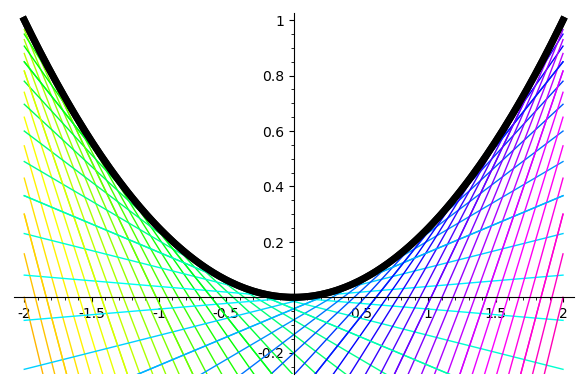
\includegraphics[width=.7\textheight,keepaspectratio=true]{./edo/solved_problem_02-05.png}
	\caption{La parábola es la envolvente de la familia de lineas rectas. }
	% solved_problem_02-05.png: 587x387 px, 100dpi, 14.91x9.83 cm, bb=0 0 423 279
	\label{fig:solved_problem_02-05}
\end{figure}




La envolvente de una familia de curvas
\begin{align}
	G(x,y,c)=0,
\end{align}
si es que existe, puede encontrarse resolviendo simultaneamente las ecuaciones
\begin{align}
	\begin{cases}
		\partial_{c}G(x,y,c) = 0\\
		G(x,y,c) = 0
	\end{cases}
\end{align}



{Solución}
\begin{enumerate}[(i)]
	%NUEVO ITEM
	\item Calculamos la parcial $
	\partial_{c}G(x,y,c) =-x+2c$

	\item Plantemos las ecuaciones
	\begin{align}
		-x+2c&=0\\
		y-cx+c^2&=0
	\end{align}

	\item Resolvemos las ecuaciones y obtenemos la solución paramética
	\begin{align}
		x=2c, y =c^{2}
	\end{align}

	\item La solución se puede reescribir como
	\begin{align}
		y = \dfrac{x^2}{4}
	\end{align}
\end{enumerate}



%DIFFERENTIAL EQUATION OF A FAMILY OF CURVES, P. 46

\begin{resuelto}
	\begin{enumerate}
		%NUEVO ITEM
		\item Trace la gráfica de varios miembros de la familia uniparamétrica $$\sett{y=cx^2}{c\in \R}$$
		\item Obtenga la ecuación diferencial de esta familia
	\end{enumerate}
\end{resuelto}



{Solución: Inciso (a)}
\begin{figure}
	\centering
	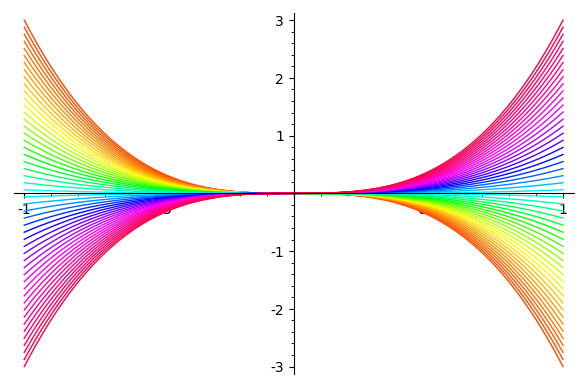
\includegraphics[height=.5\textheight,keepaspectratio=true]{./edo/solved_problem_02-06.png}
	% solved_problem_02-06.png: 587x387 px, 100dpi, 14.91x9.83 cm, bb=0 0 423 279
	\caption{Familia uniparamétrica $y=cx^2$}
	\label{fig:solved0206}
\end{figure}



{Solución: Inciso (b)}
\begin{enumerate}[(i)]
	%NUEVO ITEM
	\item  $y=cx^3 \imply y'=3cx^{2}$
	\item $c=\dfrac{y}{x^3}$
	\item $y'=3\left( \dfrac{y}{x^3} \right)x^2$
	\item $y'=\dfrac{3y}{x}$
\end{enumerate}



\begin{resuelto}

	Encuentre una ecuación diferencial para la familia biparamétrica de cónicas
	\begin{align}
		ax^{2}+by^{2}=1
	\end{align}

\end{resuelto}




\begin{proof}[Solución]

	Supongamos que $b\neq 0$.
	\begin{enumerate}[(i)]
		%NUEVO ITEM
		\item $2ax+2byy'=0$
		\item $a = \dfrac{-byy'}{x}$
		\item $\left( -\dfrac{byy'}{x} \right)x^{2}+by^{2}=1$
		\item $-bxyy'+by^{2}=1$
		\item $-b\left( xyy''+xy'^{2}+yy' \right)
		+2byy'=0$
		\item $xyy''+xy'^{2}-yy'=0$
	\end{enumerate}
\end{proof}



\begin{enumerate}
	%NUEVO ITEM
	\item  Encuentra una solución general para la ecuación diferencial $\dfrac{dy}{dx}=3x^{2}$
	\item Traza la gráfica de las soluciones obtenidas en el inciso (a)
	\item Determina la ecuación de la curva particular en el inciso (b), que pasa por el punto $\left( 1,3 \right)$
\end{enumerate}


{Solución: Inciso (a)}
\begin{enumerate}[(i)]
	%NUEVO ITEM
	\item $dy=3x^{2}dx$
	\item $\displaystyle
	\int dy = \int 3x^{2}dx$

	\item $y=x^{3}+c$
\end{enumerate}


{Solución: Inciso (b)}
\begin{figure}
	\centering
	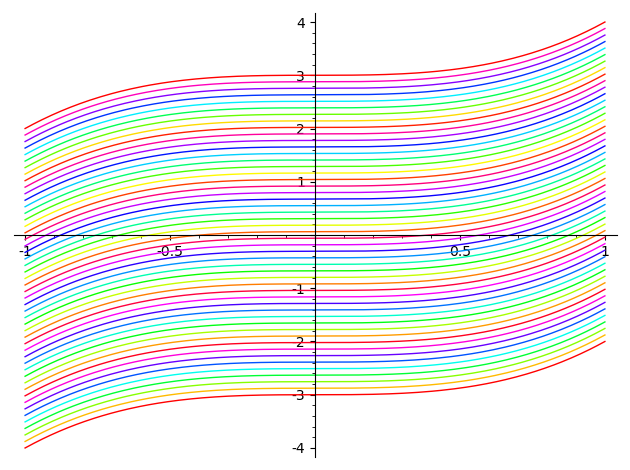
\includegraphics[height=.6\textheight,keepaspectratio=true]{./edo/solved_problem_02-08.png}
	% solved_problem_02-08.png: 630x470 px, 100dpi, 16.00x11.94 cm, bb=0 0 454 338
	\caption{Familia uniparamétrica $y=x^3+c$}
	\label{fig:solved_problem_02-08}
\end{figure}



{Inciso (c)}
\begin{enumerate}[(i)]
	%NUEVO ITEM
	\item Como la curva pasa por $(1,3)$, entonces
	$$x=1 \imply y =3$$
	\item $$
	3 = 1^{3}+c \imply c=2
	$$
	\item $y=x^{3}+2$
\end{enumerate}



\begin{resuelto}
	Resuelva el problema de condición inicial
	\begin{align}
		\begin{cases}
			y''=3x-2\\
			y(0)=2\\
			y'(1)=-3
		\end{cases}
	\end{align}
\end{resuelto}



\begin{proof}[Solución]
	\begin{enumerate}[(i)]
		%NUEVO ITEM
		\item $y'=\dfrac{3x^{2}}{2}-2x+c_{1}$
		\item $y'(1)=-3\imply
		-3=\dfrac{3}{2}-2+c_{1} \imply
		c_{1}=-\dfrac{5}{2}$
		\item $y= \dfrac{x^{3}}{2}-x^{2}-\dfrac{5x}{2}+c_2$
		\item
		$y(0)=2\imply
		c_{2}=2 \imply
		y = \dfrac{x^{3}}{2}-x^{2}-\dfrac{5x}{2}+2$
	\end{enumerate}
\end{proof}


